%# -*- coding: utf-8-unix -*-
%%==================================================
%% chapter01.tex for SJTU Master Thesis
%%==================================================

%\bibliographystyle{sjtu2}%[此处用于每章都生产参考文献]
\chapter{相关技术和国内外研究现状}
\label{chap:art_of_state}
随着容器虚拟化技术的不断发展,将容器应用到云计算中已经成为各云服务厂商的趋势。本文着重解决在容器云的环境中,以满足可用性指标为前提,通过主动式调整来加强容器云对负载变化的响应能力。在本文中,我们通过对预测负载变化来提前对服务进行调整,同时优化资源供给和放置策略来加速容器云中服务调整过程来实现容器云中的主动式调整。主动式调整主要涉及负载预测、资源供给和负载调节这三个方面。本章将从容器虚拟化技术、负载预测、资源供给和负载调节这四个要素对容器云主动式资源管理模型中所涉及的技术和国内外相关研究现状进行介绍与说明。

\section{容器虚拟化技术} 
\begin{figure}[H]
\centering
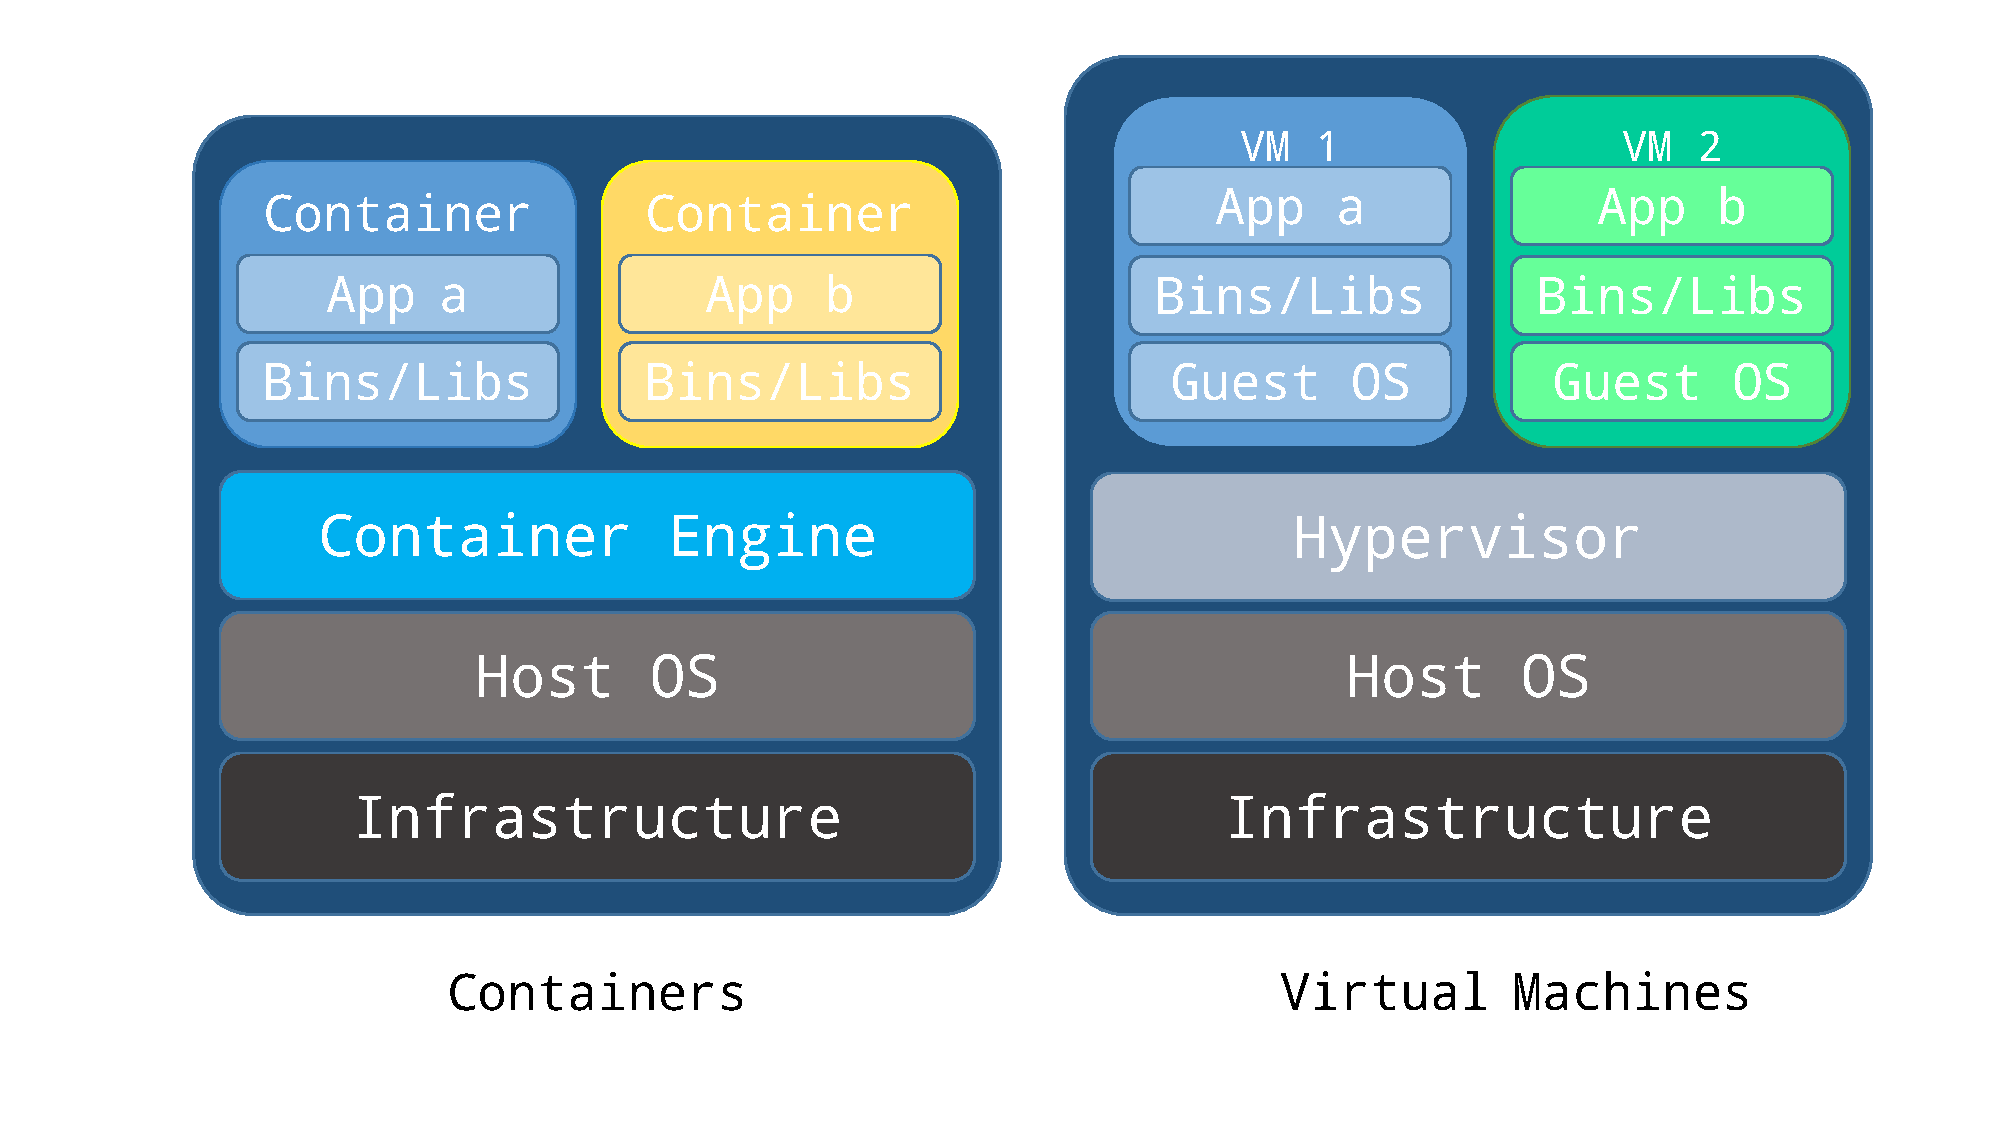
\includegraphics[width=0.9\textwidth]{./figure/container-vm}
\bicaption[fig:container_vs_vm]{容器和虚拟机架构对比}{\textbf{容器虚拟化} VS \textbf{虚拟机}}{Fig}{Containerization VS Virtual Machine}
\end{figure}
虚拟化技术作为云计算的基石,已经被广泛应用于云计算之中\cite{zhang2010cloud}。以虚拟机管理器(Hypervisor)为代表的全虚拟化技术,通过在主机操作系统之上加载额外的客户端操作系统和主机操作系统提供的特权指令来实现资源的供给和隔离。但也正是由于需要加载额外的客户端操作系统和执行特权指令所需要的开销,导致了运行时额外的资源开销和启动延迟\cite{bernstein2014containers}。相比传统的虚拟机管理器而言,容器虚拟化技术更加轻量级,可以提供更高的资源利用率并大大减少虚拟化实例的启动时间\cite{soltesz2007container}。图\ref{fig:container_vs_vm}显示了容器虚拟化技术和虚拟机之间技术框架的差异:不同于虚拟机,容器实例之间共享主机操作系统和相同的依赖库,各实例只需要单独处理各自不同的依赖库安装和环境设置。

\section{负载预测}
针对历史数据的分析和预测有很多方法,从简单的平均算法、回归算法到复杂的人工智能算法。在负载预测领域,整体上可以分为基于时间序列数据\cite{hamilton1994time}分析的预测模型和非时间序列数据的预测模型。基于时间序列数据的预测已经被广泛研究和应用在计量金融学、天气预报和地震预报等领域。经典的基于时序数据分析的预测模型有很多:
\begin{enumerate}
\item 自回归滑动平均(autoregressive moving average, ARMA)模型和差分整合移动平均自回归(autoregressive integrated moving average, ARIMA)模型,这两个模型都是基于移动平均(Moving Average, MA)模型和逻辑回归(Autoregressive, AR)模型\cite{box2015time}。这类模型受限于本身自相关系数的影响,预测结果通常相比观测值有一定的滞后性,Yang等也发现相比ARIMA模型和ARMA模型,一元线性回归模型有更高的预测精确度\cite{yang2013workload};
\item 基于移动平均模型的扩展还有指数移动平均(Exponential Moving Average,EMA)模型\cite{xiao2013dynamic}和加权移动平均(Weighted Moving Average,WMA)\cite{wu1989time},Huang等发现双重指数平滑模型因为能够反映出变化趋势,因此比起单纯的平均模型和加权平均模型由更高的预测精度\cite{huang2012resource};
\item 自回归条件异方差模型(Autoregressive conditional heteroskedasticity,ARCH)模型\cite{bollerslev1986generalized}则在应对波动形的时间序列数据场景下有出色的表现,在金融领域中被广泛应用于风险预测。Adegboyega则提出在线性模型下,ACS(Adaptive Conditional Score Models)模型相比ARCH模型和ARIMA模型有更高的预测准确率\cite{adegboyega2015dynamic};
\item 基于隐式马尔科夫模型的卡尔曼滤波(Kalman Filtering)模型\cite{goodwin2014adaptive}在短期预测中有较好的表现,但是由于该模型只是根据上一时刻的数据进行分析预测,因此并不适合周期性变化特征的场景下。Mark等发现,相比于基于简单卡尔曼滤波的预测模型,基于二次指数平滑的预测模型能提供更高的预测准确率和更少的预测开销\cite{mark2011evolutionary};
\item 成长曲线(Growth Curve)模型中成长速度随着时间增长而增长,Višnja Križanović等发现Gompertz曲线模型的预测曲线可以很好地跟随观测曲线的增长\cite{vcik2016comparison}。Lu等提出一个优化的预测模型,负载增加时使用Gompertz曲线模型进行预测,而在负载下降时使用移动平均模型来预测,提供了一定的预测准确率\cite{lu2014dynamic}。
\end{enumerate}

非时序数据的预测模型主要是基于人工智能技术的预测模型,常见的模型有人工神经网络(Artificial Neural Network)模型、支持向量机(Support Vector Machine,SVM)模型和高斯过程(Gaussian Process)模型等。除了上述模型之外,Jheng等还提出了一种基于灰度系统的负载预测模型\cite{jheng2014novel}。他们通过在灰度系统中根据时间的相关性来对未来的负载进行预测。该模型在负载增加时预测值和实际值比较相近,但是在负载下降时预测值始终高于实际值。这些人工智能模型的有点在于相比时间序列在应对周期性负载模式时预测精度较高,同时因为采用的是离线学习模式,可以对历史数据进行大量的分析。这是基于时间序列数据的预测难以做到的,但是也因为离线学习的问题,导致不能应对突发的负载变化。

Pati等提出将多层前向神经网络模型和ARIMA模型相结合,能获得相比单独的神经网络模型和单独的ARIMA模型更高的预测精度\cite{pati2014comparison}。他们将负载模型分为线性模型部分和非线性模型部分,通过ARIMA模型来得出线性模型的预测值,多层前向神经网络来得到非线性模型的预测值,然后将两者结合得到最终的预测结果。他们针对的预测对象是Debian系统的漏洞数,预测的时效性在面对随着时间迅速变化的负载场景并不适用。

Kim等选择了21个负载预测模型并对这些负载预测模型进行了评估\cite{kim2016empirical}。他们将负载的预测模型分成四个种类:简单预测模型、基于回归的预测模型、基于时间序列数据分析的预测模型和非时间序列数据的负载预测模型。其中,简单预测模型是对数据取平均值或者取最近K个数据求平均值的预测模型。根据最终的评测结果,SVM模型具有最高的预测精确度,WMA模型和ARMA模型的精确度紧随其后,简单预测模型的预测精度最差。但是SVM模型作为离线学习模型,只适用于周期性变化的场景,不能将实时的负载变化加入到之后的预测分析中,ARMA模型在历史数据较多的场景下预测分析的速度最慢,难以应对突发的变化。WMA模型和多层神经网络模型的耗时最少,但是多层神经网络模型在21个预测模型中只有中等的预测精度。

以上提及的预测模型都有着各自的优点和缺点,整体而言,基于时间序列数据分析的预测模型适用于短期变化的场景,而基于机器学习的预测模型则适用于长期的预测。但是由于现实中复杂的负载变化场景,没有任何一个通用的预测模型能满足现实中的负载预测。在本文提出的主动式容器云资源管理模型中,我们只能根据不同的负载变化场景,选择合适的预测模型并对其进行相应调整后进行负载预测。

\section{资源供给}
云计算中提出的“pay-as-you-go”模型理论上根据用户的实际需要动态分配资源,收费时则根据用户使用的实际资源总量进行计价\cite{armbrust2010view}。然而目前在实际使用中,云服务提供商都需要用户自己指定需要的资源数目,而不是用户实际的SLA\cite{patel2009service}。这导致用户常常为了确保自身的正常使用而申请过多的资源从而造成资源浪费,或者预计的资源并不足以应对实际的负载导致不能到达一开始的服务目标。为了应对上述的问题,Chaisiri等提出一个基于确定性等价式的资源供给优化算法,提供一个满足基本需要的长期资源供给方案和一个能根据负载现状立刻调整的短期资源供给方案,其中长期方案资源消耗更少,短期方案消耗更多\cite{chaisiri2012optimization}。他们的资源优化算法针对的是由用户选择云服务提供商提供资源供给方案的场景,没有从云服务提供商层面出发,使得资源供给方案不够灵活,仍然会造成较多的资源浪费。

Le等基于排队论理论,认为可以根据任务队列中任务的平均等候时间来动态的调整资源使用量\cite{le2013dynamic}。根据任务队列中当前和上一个任务之间的出队时间差当作任务的运行时间,基于M/M/1队列模型根据虚拟机的CPU计算能力计算任务队列中每个任务所需要的虚拟机数量,从而决定对虚拟机资源池进行伸缩。这个方案整体目标是让所有任务可以在用户设定的截止时间之前完成,只考虑了CPU的消耗,没有考虑存储和网络带宽等其他因素,同时资源调整的粒度仍然是虚拟机粒度,没有考虑资源伸缩需要的开销和资源的浪费。

Wu等通过将SLA映射到云服务的服务质量(Quality of Service,QoS),得到一个基于SLA的资源供给模型\cite{wu2014sla}。该模型基于最适配原则提出了两个优化的资源供给算法。这两个算法相比单纯的查找最优适配算法,减少了虚拟机迁移的开销,总体上提高了用户SLA的满足率。第一个算法的优化对比算法中针对找不到相同类型请求的合适虚拟机实例是通过新建虚拟机实例来实现的,因此实际中的优化优先。第二个算法的问题则是需要通过大量的冗余来规避虚拟机迁移造成的额外开销,随着请求种类的增加冗余也会大量增加,使云服务提供商产生额外的成本。

针对数据迁移需要跨物理机房的场景,Chase等提出一个基于随机规划模型的资源供给方案\cite{chase2017joint}。他们将虚拟机迁移所需要的带宽作为资源供给算法计算的一部分,利用场景树缩减算法来尽可能快的提供一个合理的启发式结果。但是该模型没有考虑虚拟机迁移过程中网络传输的耗时,同时由于现实网络环境的异构性,导致对该问题的分析极其复杂。

Guo等针对空间上分离的云服务提供商,提出一个基于排队论中G/G/1模型的主动式资源供给方案\cite{guo2016geoscale}。通过检测不同地区的云服务中任务的等待时间和平均服务时间从而得出每个云服务中需要的虚拟机数目,然后根据虚拟机数目对各云服务中的实例进行伸缩,利用各个云服务的本地行来降低不同云服务之间的迁移开销。然而这个方案直接对虚拟机进行水平伸缩,没有考虑使用垂直伸缩来降低迁移操作本身的开销。

以上所说的资源供给方案都是针对虚拟机进行的优化,在设计中并没有考虑容器的特性。

\section{负载调节}
负载均衡作为在多计算资源间分配负载,实现最优化资源使用和提高吞吐量等目标的技术,在国内外已经有广泛的研究。Randles等对三种分布式负载均衡方案进行了比较和讨论\cite{randles2010comparative}。该论文探讨的三种分布式负载均衡算法在伸缩性上有较好的表现,但是没有考虑系统伸缩过程中对吞吐量造成的影响和开销。

Hu等提出一个基于遗传算法的负载均衡分配方案\cite{hu2010scheduling}。通过遗传算法得到当前环境下最优的负载分布,然后根据最优的负载分布找到从当前状态调整过去开销最少的策略则是满足目标的负载均衡方案。然而该方案假定所有的虚拟机服务能力始终一致,没有考虑服务器垂直伸缩的问题。同时基于遗传算法,最后得出的解可能只是局部最优解而不是全局最优解。

Alizadeh等针对数据中心网络流量巨大的现状,设计并实现了一个基于网络层拥塞感知的分布式负载均衡模型\cite{alizadeh2014conga}。由于数据中心的特性,采用中心化的负载均衡方案将导致负载均衡模块难以应对巨大的流量请求,从而成为性能瓶颈。这篇论文从传统的基于网络流量的角度设计了一个分布式的负载均衡器,但是没有考虑到数据中心内实际运行的服务器本身的处理能力,可能出现虽然某些服务器带宽资源充足但是其他诸如CPU能力或者内存等资源不充足的场景,这样单纯按照带宽进行分配反而会造成资源分配不合理,导致性能的下降和资源的浪费。

Wang等参照负载均衡中负载窃取算法,提出一个面向数据敏感的基于自适应负载窃取算法的负载均衡模型\cite{wang2014optimizing}。该论文建立了一个去中心化的负载均衡模型,提供了更高的健壮性和可伸缩性,但是主要针对的是数据敏感的场景,并不具有普适性。该模型研究的场景下所有的虚拟机都是相同的服务能力,也没有考虑不同虚拟机之间实际服务能力不同的问题。

以上论文大多设计了分布式的负载均衡方案,提升了可伸缩性和健壮性,但是也基本都是只以带宽资源作为负载均衡的调节基准,并没有考虑如何应对负载动态变化的问题。随着过去几年云计算的急速发展,通过更好的调度任务和分配资源来应对负载变化的方案也在被广泛研究。Li等研究了虚拟机在集群中的成本最小化放置方法,并提出了一个权衡了网络流量和物理设备成本的最优化算法\cite{li2014let}。Peng等构建了一个基于文件块的虚拟机镜像分发网络,从而加速了虚拟机实例的部署和启动速度\cite{peng2012vdn}。Harter等构建了基于中央式存储服务的存储驱动Slacker,加速了容器在集群中部署和启动,但是这需要额外的网络文件系统(NFS)存储服务器提供基于文件系统层面的专门支持\cite{harter2016slacker}。Gog等基于最小费用最大流(MCMF)算法提出了中央式调度器Firmament来降低放置过程的延迟\cite{gog2016firmament}。Kaewkasi等基于蚁群算法提出一个新的启发式算法来确定Docker swarm集群中任务和资源的分配和管理,从而提升了集群整体的性能\cite{kaewkasi2017improvement}。这些方案提升了云环境下对负载变化的响应能力,然而,以上方案都忽视了资源和任务的调整对可用性的影响。

\section{本章小结}
对于云服务提供商而言,如何做到在保证满足SLA的同时尽可能提高资源使用率,减少资源浪费从而降低整体成本仍然是一个重要的问题。将这个问题拆分成两个子问题,则分别是满足SLA和提高资源使用率。基于预测的方案可以提前采取伸缩控制资源供给应对负载的变化,避免由于负载变化来不及调整导致违反SLA;而为了提高资源使用率,可以引入负载均衡的策略。但是目前相应的方案仍然存在很多问题:首先,现有的云资源供给方案大多基于虚拟机这一虚拟化技术,相比轻量级的容器虚拟化技术而言,虚拟机间的资源迁移操作本身耗时更长,额外的资源开销更多;其次,已有的负载均衡方案大多是从网络流量本身的角度考虑的,没有考虑虚拟机除带宽资源以外能提供的服务能力;然后,已有的负载优化方案没有考虑容量调整操作本身耗时带来的影响,使得整体的调整总是落后于负载的变化了;最后,针对容器集群的解决方案都忽视了用户对可用性的约束。本文为了解决上述问题,提出一个基于容器的主动式云负载均衡模型。和传统的根据负载实时状态进行集群伸缩的被动式调整策略不同,该模型试图通过对负载进行监测后预测将来一段时间的负载,然后根据预测的负载提前对容器云进行伸缩,在保证服务本身可用性的前提下,减少应对负载变化所需要的延迟,提升容器云整体的性能。